\chapter[SCP-022 停尸房]{
    SCP-022 The Morgue\\
    SCP-022 停尸房
}

\label{chap:SCP-022}

\begin{figure}[H]
    \centering
    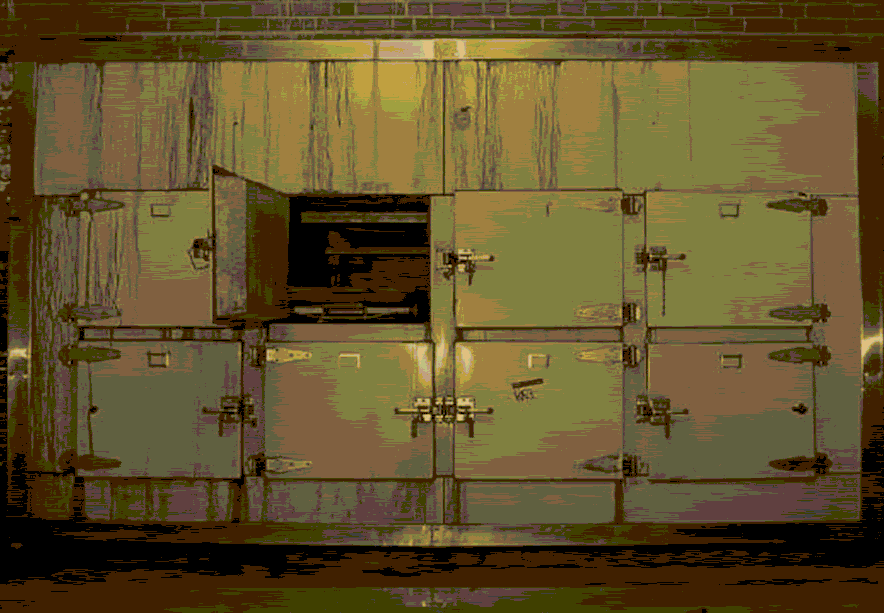
\includegraphics[width=0.5\linewidth]{images/SCP.022.png}
    \caption*{通過安全摄像头所拍攝的SCP-022}
\end{figure}

\bb{项目编号:} SCP-022

\bb{项目等级:} Euclid

\bb{特殊收容措施:} 在编号022-827的意外发生后,已加装保管库大门来密封SCP-022。除非SCP-022-1现身,不然保管库大门必须一直锁着。 SCP-022原本的门已经在意外022-827中被破坏,而每次尝试更换都以失败告终。已经安装安全摄像头来监察会否出现SCP-022-1。

在SCP-022-1出现时,在它离开SCP-022后应立即启动自动焚化系统,之后可以开启保管库大门来清理残留物。如果自动焚化系统没有消灭SCP-022-1,快速反应团队应该进入SCP-022并摧毁它。除了4级人员下达的实验指令外,活人在任何情况下都不能进入SCP-022。4级人员可以下令活捉或禁锢SCP-022-1,不过它们不能移出SCP-022的防护设施。

\bb{描述:} SCP-022是个位于大不列颠[编辑]医院地下室的太平间。直到198█,该太平间都没有报告异常事件。第一次收到异常活动的报告是在198█年9月,然后该区域很快就被基金会隔离,并在放出官方说法后将整个大楼净化。此特殊行为的原因尚在调查当中。

每隔一段时间,太平间内的一个随机抽屉会打开,并展示出一个躺在台子上,被盖尸布所覆盖的尸体。约六分钟后,尸体会移动并尝试离开太平间。此时该尸体会被标记为SCP-022-1。在某些情况下,SCP-022-1会损坏或是成功离开SCP-022,甚至从台子上坐起来。在这种情况下,SCP-022-1通常会摔倒并抽搐直到到达活动时限。假如SCP-022-1在时限到达后还在台子上,台子会收回去抽屉并关上。报告表示接着会出现类似烧毁人体组织的气味。

暂时还不清楚SCP-022-1的活动能源。SCP-022-1并不会呼吸、进食或睡眠,而它们也没有体温。分析SCP-022-1后发觉没有异常的器官或化学成份,它们似乎只是普通的人类尸体。

SCP-022-1同时具有超越常人的力量。经过直接测试后被证实存在问题,研究人员估计在和一般的人类同等情况下,上升力大约提升500N(112磅) 。正在进行分折以确认这是来自于未知的力量来源或是独立情况。

当SCP-022-1的身体部位被切断,具有最大质量的部份会继续活动,其他的部份则静止。破坏心脏或头部并不能消灭SCP-022-1,其他部份跟四肢都会继续活动。只有完全破坏所有组织才能消灭SCP-022-1。独处时SCP-022-1会很容易到达活动时限,所有迹象都显示它会再次成为一具普通的尸体。所耗时间视乎SCP-022-1的损伤及腐烂程度,已知为2天至3个星期。

调查发现,已知的SCP-022-1的躯体都符合城市内的太平间所报告的遗失尸体。目前正在研究这种转移机制。

已证实不可能增加任何物体至SCP-022。任何进入SCP-022的物体都会很快在穿过门后消失,且不留下任何痕迹。这包括任何无机物及生物标本。参阅附录022-001及022-002。

假如SCP-022-1拥有一个正常运作的嘴巴、舌头及气管,那它就能跟研究人员沟通。参阅\hyperref[sec:DOC-interview-log-022-751]{采访日志 022-751}。

\bb{附录022-001:} 已提交删除南边墙壁的一部份来增加SCP-022的入口的申请。申请等待批准。

\bb{附录022-002:} 在SCP-022的正下方发现一堆物质,它似乎包含除了人类外所有放到SCP-022的材料。所有材料都出现破裂及磨损。金属部份被严重锈蚀,生物分解的各个阶段的所有部分。经测试后发现物体放置进SCP-022后会在183秒后会以以上情况出现,而人类进入后则不会出现以上情况。而是似乎被融入太平间中,并有可能成为SCP-022-1实体。

\section{采访日志022-751}

\label{sec:DOC-interview-log-022-751}

以下对话大致使用相同的方式,SCP-022-1通常都是歇斯底里,直到基金会人员都能够安抚\slash 拘束他们。这些部分被省略了。

\bb{日期:}198█年3月█日

受访者:SCP-022-1-2

采访者:██████博士

注记:SCP-022-1-2为第二位被基金会所发现的例子,而第一位被基金会特工发现后消灭。SCP-022-1-2有着亚州男士的身体,年龄约为43,其胸部被缝合了,显示它曾被尸检。

\begin{scpbox}

\bb{[对话开始]}

██████博士:请说明你的身份。

SCP-022-1-2:我…我的名字是约翰 █████████。 TMD到底发生什么事?

██████博士:约翰,这就是我们正在努力搞清楚的。你是如何得到这个…状态?

SCP-022-1-2:我…我不知道。我记在驾驶自己的车回家…由那个…算了。我在驾车,然后撞车了。

██████博士:接着发生什么事?

SCP-022-1-2:什么都没有!我就在这里醒来了!拜托…这一定要[不知所云]。

██████博士:所以你记得发生了交通意外,然后在这太平间内醒来?你对如何到达这里有什么想法吗?

SCP-022-1-2:我没有来这里!你清楚吗?这不是我!我不是我!

██████博士:“我不是我”是什么意思?

此时SCP- 022-1-2情绪非常激动以至必须被物理拘束,由于SCP-022-1的力量增加而需要6个特工去实行。最终SCP-022-1-2变得冷静并继续进行访谈。

██████博士:现在,请你解释你想表达的是?

SCP-022-1-2:这。不。是。我。 我可以看到在钢材上的倒影。我可不是一个年老的亚州傻逼! 这不是我!

\bb{[对话结束]}

\end{scpbox}

在上述对话之后,SCP-022-1-2开始以头撞墙。一旦试图控制,对象会发出难以理解的尖叫持续好几个小时。安静下来后它仍会继续挣扎,但显然无法说话,直到六天后才完全停止活动。在这段时间内,对象以正常速度继续腐坏。在这次对话后的身体检查无法确定其死亡原因,因为许多内部器官已消失。此次手术\slash 尸检与之前的结果相比,只是新发现了一处气管损伤。

\bb{日期:}198█年3月█日

受访者:SCP-022-1-5

采访者:██████博士

注记:D -5619被送进SCP- 022后失踪,而SCP-022-1-5 在不久后出现。 SCP-022-1-5 有着约12岁女性的身体,但失去右臂和大部份的躯干。在SCP-022-1-3事件之后,所有SCP-022-1都必须被物理拘束后才能接触重要人士,SCP-022-1-5也不例外。

\begin{scpbox}

\bb{[对话开始]}

██████博士:请说出你的姓名。

SCP-022-1-5:你们这些混蛋对我TMD做了些什么事?

██████博士:请说出你的姓名。

SCP-022-1-5:你TMD对我做了些什么事!?

██████博士:我们什么都没对你做过,现在请说出你的姓名。

SCP-022-1-5:你TMD知道我是谁!

██████:那请你再次提醒我。

SCP-022-1-5:我是刚刚被你TMD的小白鼠。别告诉我你已经忘记了,混蛋博士。

██████:…你是D-5619?

SCP-022-1-5:在这个肉体内。然后为了你的数据,蠢驴,我的名字是[绝密]!现在TMD把我变回来,不然我對上帝发誓我会扭断你聪明的小脑袋!

\bb{[对话结束]}

\end{scpbox}

接着██████博士向SCP-022-1-5提问了数个问题以确认它的身份。虽然确认了它是D-5619,但从SCP-022-1-5身上没有收集到其他有用资料。它被保存在一个牢房直到到期两天后到达活动时限。三个星期后,SCP-022-1-7以D- 5619的身体出现。在一个简短的对话后,SCP-022-1-7声称它是一个89岁的女性。

